\documentclass[a4paper,12pt]{article}
\usepackage[a4paper, total={7in, 9in},headheight=10mm]{geometry}
\usepackage{graphicx}
\usepackage{fancyhdr}
\usepackage{xcolor}
\usepackage{pifont}
\usepackage{color,soul}
\usepackage{chngcntr}
\usepackage[hidelinks]{hyperref}
\usepackage{caption}
\captionsetup[figure]{labelformat=simple, labelsep=period}
\counterwithin{figure}{section}


\fancyhf{} 
% Define the blue color
\definecolor{myblue}{RGB}{0,0,255}
\pagestyle{fancy}
\fancyhead[L]{
	\quad	
\includegraphics[trim=0cm 0 14cm 0cm, clip, width=0.1\textwidth]{dct-logo}
}
\fancyhead[R]{Rev A1-00\quad}
\fancyhead[C]{Development and Test Plan}
\fancyfoot[C]{Proprietary \& Confidential }
\fancyfoot[L]{\textcolor{myblue}{www.dicortech.com }}
\renewcommand{\headrulewidth}{1pt}
\renewcommand{\footrulewidth}{1pt}
\renewcommand{\headwidth}{480pt}

\fancyfoot[R]{\thepage}

\begin{document}
	\pagenumbering{roman}
	
	\begin{titlepage}
		\begin{flushleft} % Left-align the image and the text
		
\includegraphics[trim= 0cm 0cm 0cm 0.2cm, clip, width=0.35\textwidth]{dct-logo}\quad % Add a horizontal space
			\begin{minipage}[b]{0.6\textwidth} % Adjust width as needed
				\raggedleft % Aligns text to the right
				\normalsize % Adjust font size as needed
				Rev A0-00 \quad \\
				$10^{th}$ July 2024 \
			\end{minipage}
		\end{flushleft}
		
		
		\vspace{6cm} % Adjust vertical space as needed
		\begin{center} % Center the title
			\Huge % Adjust font size as needed
			\textcolor{blue}{\textbf{DS\_CSLI\_MSEOVS}}\\
			\textbf{Development and Test Plan}
			%	\textbf{Product Overview and Architecture Design}
		\end{center}
		
		%In order to show contact details uncomment below lines
		%\vfill %33ll the vertical space
		%	\raggedright % Aligns text to the left
		%	\textbf{Contact Details:} \\
		%	Thomas S \\
		%	thomas@dicortech.com \\
		%	Digital Core Technologies Pvt. Ltd. \\
		%	\textcolor{blue}{www.dicortech.com} % Change the color to blue
	\end{titlepage}
	
	\newpage
	
	
	\textbf{Revision History:} \\
	\\
	\begin{tabular}{|l|l|l|l|}
		\hline
		Date & Version \# & Description & By \\
		\hline
		10th July 2024 & A0-00 & Draft & Richu Bini \\
		\hline
		& \  & \ & \  \\
		\hline
	\end{tabular}
	\newpage
	\tableofcontents

	\listoffigures
	\newpage
	

	
	\pagenumbering{arabic}
	\newpage
	\section{Development and Test Plan}
	
	\subsection{Software }
	
	\begin{figure}[h]
		\centering
		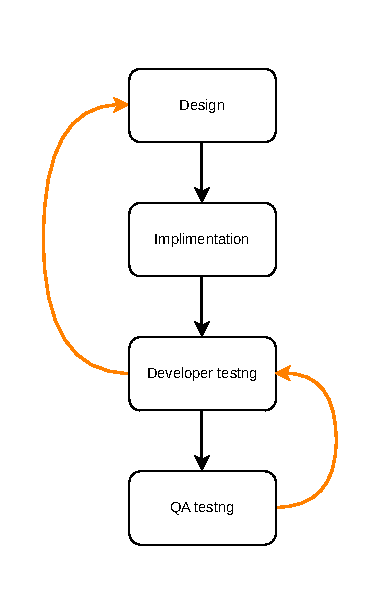
\includegraphics[width=0.3\textwidth]{d-t} % Ensure you have yolo-architecture image in the same directory
		\caption{Work flow of development Phase}
		\label{fig:Work flow of development Phase}
	\end{figure}
	
	 \subsubsection{Design}
	
	This initial phase focuses on designing both the software and hardware modules for the product. Additionally, comprehensive test plans are created for each individual module to ensure thorough testing throughout the development process.
	
	 \subsubsection{Implementation}
	
	During this phase, the development team translates the designs into functional software modules and hardware elements.
	
 \subsubsection{Developer Testing}
	
	Following development, each module undergoes rigorous testing by the developers themselves. Any issues identified trigger a redesign, implementation, and retesting cycle for the affected module. This iterative process ensures that each module functions as intended before being integrated with the entire system.
	
 \subsubsection{QA Testing}
	
	Once individual module testing is complete, the fully integrated system, encompassing both software and hardware, is then delivered to a dedicated Quality Assurance (QA) team for comprehensive testing. The QA team utilizes the pre-defined test plans created during the design phase and the new test cases that the tester added to meticulously test all functionalities and features of the product. If any problems are discovered, the QA team reports them to the development team. The development team then addresses the identified issues, fixes them, and resubmits the product to QA for further testing. This iterative process continues until the product is free of defects and meets all quality standards. Upon successful completion of QA testing, the development team initiates the product release procedure.
	\\
	\\
	\noindent
	\subsection{Hardware }
	\noindent
	The following is the list of processes that we follow for the development of the hardware system in order.
	\begin{enumerate}
		\item Requirement analysis
		\item HW design documentation
		\item HDD review and update
		\item Schematic Design
		\item Schematic review and update
		\item PCB Floor plan
		\item PCB placement review and verification from mechanical side
		\item Layout routing
		\item Layout routing  review and update
		\item Draft Gerber release
		\item Draft gerber review and update
		\item Gerber release
		\item PCB fabrication and assembly
		\item Board bring up and testing
	\end{enumerate}

\newpage
	\subsection{Detailed Development Plans With Schedules}
	\subsubsection{Hardware}
\begin{tabular}{|l|l|}
	\hline
	\textbf{Task} & \textbf{Duration} \\
	\hline
	Hardware Design & PDR+ 3 weeks \\
	\hline
	Schematic Design & PDR + 4 weeks \\
	\hline
	PCB Layout design & PDR + 7 weeks \\
	\hline
	Gerber Release & PDR + 8 weeks \\
	\hline
	FAB and Assembly & PDR + 14 weeks \\
	\hline
	Basic Bring up and testing & PDR + 16 weeks \\
	\hline
\end{tabular}

	\subsubsection{Software}
	The following are the milestones and the schedules of software development and testing.\\
	\textbf{Milestone 2}\\

\noindent
\begin{tabular}{|l|l|}
	\hline
	\textbf{Task} & \textbf{Duration} \\
	\hline
	Detailed Software Design & PDR + 2 weeks \\
	\hline
	Preparation for trials & PDR + 4 weeks \\
	\hline
	CLASS review & PDR + 4 weeks \\
	\hline
	Setup basic camera ready for capturing the dataset & PDR + 5 weeks \\
	\hline
	PTZ and LRF interfacing & PDR + 6 weeks \\
	\hline
	Setup communication node for interaction with HMI/Custom PC application & PDR + 7 weeks \\
	\hline
	Actual trials for capturing images in different environment & PDR + 10 weeks \\
	\hline
\end{tabular}\\
\newline
\noindent
	\textbf{Milestone 3}\\
	
	\noindent
	\begin{tabular}{|l|l|}
		\hline
		\textbf{Task} & \textbf{Duration} \\
		\hline
		Object detection and tracking algorithms implementation phase-1 & PDR + 13 weeks \\
		\hline
		Detection trial -1 & PDR + 14 weeks \\
		\hline
		Object detection and tracking algorithms implementation phase-2 & PDR + 16 weeks \\
		\hline
		Detection trial -2 & PDR + 17 weeks \\
		\hline
	\end{tabular}
	\\
	\newline
	\noindent
	\textbf{Milestone 4}\\
	
\noindent
\begin{tabular}{|l|l|}
	\hline
	\textbf{Task} & \textbf{Duration} \\
	\hline
	QA Testing in DCT & PDR + 18 weeks \\
	\hline
	QA Testing in field & PDR + 19 weeks \\
	\hline
	QA Testing at CSAS & PDR + 20 weeks \\
	\hline
\end{tabular}

	\newpage
	\subsection{Types of Test}
	
	\subsubsection{Hardware Tests}
	
	\begin{itemize}
		\item \textbf{Baisc HW bring up and test: }
		Will check all the basic functionality and interface testing.
		\item \textbf{HW protection test:}
		We will test the voltage protection conditions. 
		\item \textbf{EMI /EMC test: }
		Applicable for the Surface ship as per the MIL-STD-461E 
		
	\end{itemize}
	
	\subsubsection{Mechanical Tests}
	\begin{itemize}
	\item \textbf{Environmental stress test : }
	Applicable as per MIL-810G 
	\item \textbf{IP65 testing : }
	IP65 testing
	\end{itemize}
	\subsubsection{Software Tests}
		\begin{itemize}
			\item \textbf{Unit test:}
			Will verify that all modules are individually working by providing specific inputs and handling errors correctly.
			\item \textbf{Integration testing:}
			Will check the interactions between the SW modules and the interaction between the SU and PU to ensure they are working correctly, and verify that the software functions properly.
			\item \textbf{System test:}
			Verifies all the features are working correctly 
		
		\end{itemize}

	 
	\subsection{Purpose and Expected Results of Test}
	
	\subsubsection{Hardware and mechanical testing expected results}

	\begin{itemize}
		\item \textbf{Baisc HW bring up and test: }\\
		\textbf{Purpose:} The bringup test is to test hardware is working correctly. It should test functionality and interface are workig correctly.\\
		\textbf {Expected result:} basic functionality and interface are workig correctly.
		\item \textbf{HW protection test:}\\
		\textbf {Purpose:} This test is to check the hardware is able to withstand the voltage protection conditions.\\
		\textbf {Expected result:} The hardware withstand the voltage protection conditions without any damage. 
		\item \textbf{EMI /EMC test: }\\
		\textbf {Purpose:} This test is to ensure that electronic devices operate correctly in their intended environment without causing or being affected by unwanted electromagnetic interference.\\
		\textbf {Expected result:}  That the device meets all emission limits and immunity criteria specified by MIL-STD-461E. 
		
		
	\end{itemize}
	
	\subsubsection{Mechanical testing expected results}
		
	\begin{itemize}
		\item \textbf{Environmental stress test : } \\
		\textbf{Purpose:} 	Performed on electronic devices and systems to ensure they can operate correctly and reliably under extreme environmental conditions. These conditions can include variations in temperature, humidity, vibration, shock, and other environmental factors that the device might encounter during its lifecycle.\\
		\textbf {Expected result:} That the device meets all the above tests as per  MIL-810G
		\item \textbf{IP65 testing : }\\
		\textbf {Purpose:} This test is to assess the degree of protection provided by enclosures of electronic and electrical devices against the intrusion of solid objects and water.\\
		\textbf {Expected result:}  That the device meets all criteria specified by IP65
	\end{itemize}

	\subsubsection{Software testing expected results}
	
		\textbf{Unit testing :}
		\\
		The expected result of unit testing is to verify that individual software modules function correctly in isolation.
		\begin{itemize}
			\item The module produces the correct output for a given set of valid inputs.
			\item The module handles invalid inputs as expected (e.g., throws errors, returns specific values).
			\item The module behaves according to its intended design and doesn't exhibit unexpected behavior.
		\end{itemize}
	\textbf{Integration testing :}
	\\
	The expected outcome of integration testing is to confirm that individual software modules function together seamlessly once combined.
	\begin{itemize}
		\item All features outlined in the project requirements work correctly across various scenarios.
		\item The application operates efficiently, meeting performance benchmarks for speed and stability.
		
	\end{itemize}

	\textbf{System testing}
\\
The expected result of system testing is to verify the entire software application functions as a cohesive unit and meets all requirements.

\begin{itemize}
	\item The module correctly share and interpret data.
	\item The module trigger each other in the correct sequence.
	\item Errors propagate and are managed properly to prevent crashes.
	\item Module interfaces communicate smoothly without conflicts.
	
\end{itemize}
		
	
	\subsection{Test Plans and Methodologies}
	\subsubsection{Hardware}
	
	\begin{itemize}
		\item Baisc HW bring up and test :
		Will check all the basic functionality and interface testing. Methodologie for testing is Manual testing 
		\item HW protection test : 
		We will test the voltage protection conditions. Methodologie for testing is Manual testing 
		\item EMI /EMC test : 
		Applicable for the Surface ship as per the MIL-STD-461E Methodology for testing is in accordance with the EMI/EMC test environment.
		
		
		
	\end{itemize}
	\subsubsection{Mechanical}
	 \begin{itemize}
	 	\item Environmental stress test :
	 	Applicable as per MIL-810G   Methodology for testing is as per environment stress test conditions
	 	\item IP65 testing : 
	 	IP and Ingress Testing. Methodology for testing is as per IP test environment conditions
	 \end{itemize}
	\subsubsection{Software }
	Software development, testing includes unit testing, integration testing, and system testing. Unit testing verifies individual software modules by providing specific inputs and checking if the outputs match the expected results. Integration and system testing focus on how these modules interact and ensure the entire software behaves correctly
	\newline
	\textbf{Unit testing :} \newline
	During unit testing, each software block undergoes rigorous testing to ensure its functionality. The following test plans outline the procedures for each software module.
	\\
	\begin{enumerate}
		\item \textbf{\textit{Target Tracker}}
		\begin{itemize}
			\item \textit{Object Tracking:}
			The unit test provides an object ID as input and verifies if the camera successfully tracks the designated object.
			\item \textit{IP Joystick PTZ Control:}
			The test simulates a joystick command and confirms the PTZ unit (Pan-Tilt-Zoom) moves accordingly.
			\item \textit{Slew to Cue API:}
			The unit test injects API calls to move the PTZ to a specific location and validates its successful movement based on the provided commands.
		\end{itemize}
		\item \textbf{\textit{Video Processor}}
		\begin{itemize}
			\item \textit{Fusing video:}
			During unit testing, decoded daylight and thermal video are input along with the fusion percentage to verify if the output is the fused video. The process also checks how the fusion percentage changes by varying the fusion percentage values.
			\item \textit { Saving video and snapshots :}
			This unit test verifies saving video and capturing snapshots. It checks if the video is saved in the correct format and location, and throws errors for invalid data. 
			\item \textit{Thermal object detection:}
			This unit test assesses thermal object detection. It feeds the system thermal image data and checks the output for accuracy. The test verifies if bounding boxes are correctly drawn around detected objects and classification labels are assigned correctly. It also includes scenarios with no objects, varying object sizes, and corrupted data to ensure the system functions as expected under different conditions.
			\item \textit{Daylight object detecting:}
			This unit test assesses daylight object detection. It feeds the system daylight image data and checks the output for accuracy. The test verifies if bounding boxes are correctly drawn around detected objects and classification labels are assigned correctly. It also includes scenarios with no objects, varying object sizes, and corrupted data to ensure the system functions as expected under different conditions.
			\item \textit{Metadata saving and streamin with time stamp:}
			The unit test  ensures that the system correctly streamed metadata with timestamps, and saves metadata accurately in the desitrd location. 
			\item \textit{Video encoding and streaming:}
			This unit test verifies video encoding and streaming functionality. It feeds the system raw video data and  ensuring correct encoding with designated settings, successful stream initiation using the RTSP protocol, and proper authentication before making the RTSP stream available for viewing.
			
			
		\end{itemize}
		
		
		\item \textbf{\textit{Comms and Alerter}}
		\begin{itemize}
			\item \textit{Metadata Creator:}
			This unit test verifies that all communication with the NMEA devices is working perfectly and checks if the system can receive the object detection metadata. Then verifies that the detected object class, bounding box coordinates, confidence rate, and the position of the object relative to the radar data are added correctly.
			
			\item \textit{Collision alerter:}
			This unit test will verify that the radar data is being received correctly. It will then simulate a collision detection scenario and check whether the collision is detected accurately.
			
			
			
		\end{itemize}
		
	\end{enumerate}
	
	\noindent
	\textbf{Integration testing :}
	\newline
	Focuses on how these modules work together, ensuring they interact smoothly once combined. Integration testing examines the interaction between software modules and also the SU to PU intractions, ensuring they work together smoothly.
	\begin{itemize}
		\item \textit{Data Exchange: }
		Verifying modules share data correctly and interpret it properly.
		\item \textit{Control Flow:}
		Ensuring modules trigger each other’s functions in the correct sequence.
		\item \textit{Error Handling: }
		Checking if errors are properly propagated and managed to prevent cascading failures.
		\item \textit{Interface Compatibility: }
		Confirming that modules communicate through defined interfaces without conflicts.
	\end{itemize}
	
	\noindent
	\textbf{System testing}
	\newline
	Examines the complete application as a whole, verifying it functions as intended and meets all requirements.System testing acts as the final quality check for the entire software application.system testing identifies and addresses any critical issues before the application is deployed to real users. In this test all the fearures of the product are tested and verified.
	\\
	\noindent
	\\
	\textbf{Methodologies}
	\\
	All the software testing are done manually.
	\newline
	
	\subsection{Test Reporting}
	
	The test reporting will be comprehsnsive document that contain all the test cases and the test report that will be added afther the QA testing.
	
	\subsection{Testing and Compliance}
	To be done along with mechanical info updation

\end{document}
